% !TEX program = pdflatex
\documentclass[conference]{IEEEtran}
\IEEEoverridecommandlockouts

\usepackage{cite}
\usepackage{amsmath,amssymb,amsfonts}
\usepackage{algorithmic}
\usepackage{graphicx}
\usepackage{textcomp}
\usepackage{xcolor}
\usepackage{booktabs}
\usepackage{multirow}
\usepackage{tikz}
\usepackage{pgfplots}
\pgfplotsset{compat=1.18}
\usetikzlibrary{positioning,arrows.meta,fit,calc,patterns,decorations.pathreplacing}
\usepackage{balance}
\usepackage{url}
\usepackage[hidelinks]{hyperref}

\def\BibTeX{{\rm B\kern-.05em{\sc i\kern-.025em b}\kern-.08em
    T\kern-.1667em\lower.7ex\hbox{E}\kern-.125emX}}

\begin{document}

\title{An Energy-Efficient RISC-V GEMM Co-Processor\\with On-Chip Requantization for Edge AI Inference}

\author{\IEEEauthorblockN{1\textsuperscript{st} Aryan}
\IEEEauthorblockA{\textit{dept. name of organization (of Aff.)} \\
\textit{name of organization (of Aff.)}\\
City, Country \\
email address or ORCID}
\and
\IEEEauthorblockN{2\textsuperscript{nd} Debargha}
\IEEEauthorblockA{\textit{dept. name of organization (of Aff.)} \\
\textit{name of organization (of Aff.)}\\
City, Country \\
email address or ORCID}
\and
\IEEEauthorblockN{3\textsuperscript{rd} Arihant}
\IEEEauthorblockA{\textit{dept. name of organization (of Aff.)} \\
\textit{name of organization (of Aff.)}\\
City, Country \\
email address or ORCID}
}

\maketitle

% ============================================================
% ABSTRACT
% ============================================================
\begin{abstract}
Edge AI inference demands energy-efficient matrix multiplication hardware, yet general-purpose processors are orders of magnitude too slow for real-time deployment at milliwatt-scale power budgets. We present a lightweight General Matrix Multiplication (GEMM) co-processor tightly integrated with a PicoRV32 RISC-V core via four custom instructions. The accelerator features a parameterizable $8\times8$ output-stationary systolic MAC array with 48-bit accumulators, a hardware tiling engine for arbitrary matrix dimensions, a double-buffered scratchpad with overlapped DMA and computation, and a novel 32-bit accumulator output mode that enables full CPU-side requantization---eliminating the need for offline precomputation in quantized neural network inference. Implemented on a Xilinx Artix-7 FPGA, the complete System-on-Chip consumes 6{,}287 LUTs (9.9\%), 70 DSP48E1 blocks, and 199\,mW total power at 91.7\,MHz. The co-processor delivers up to 212$\times$ speedup over software GEMM in int8 mode and 100$\times$ in 32-bit accumulator mode, achieving a peak throughput of 5.87\,GOPS at 52\,GOPS/W energy efficiency. We demonstrate end-to-end MNIST digit recognition using a TFLite-quantized convolutional neural network with on-chip requantization, achieving bit-exact correctness across 60 verification patterns.
\end{abstract}

\begin{IEEEkeywords}
RISC-V, GEMM accelerator, edge AI, systolic array, quantized inference, FPGA, co-processor, neural network
\end{IEEEkeywords}

% ============================================================
% I. INTRODUCTION
% ============================================================
\section{Introduction}

The proliferation of deep learning at the network edge---in wearable health monitors, autonomous micro-robots, and always-on keyword spotters---requires inference engines that operate within strict milliwatt power envelopes while sustaining acceptable throughput~\cite{banbury2021mlperf}. At the computational core of these workloads lies General Matrix Multiplication (GEMM), which accounts for over 90\% of the arithmetic in convolutional and fully connected neural network layers~\cite{jouppi2017datacenter}.

General-purpose microcontrollers, even those implementing the RISC-V RV32IM instruction set with hardware multiply support, remain fundamentally inefficient for dense matrix arithmetic: a software $16\times16$ GEMM on the PicoRV32 core consumes over 254{,}000 clock cycles. Cloud-oriented accelerators such as GPUs and Google's TPU~\cite{jouppi2017datacenter} deliver high throughput but at power levels ($>$2\,W) incompatible with battery-powered edge devices. There is a clear gap for sub-200\,mW accelerators that can be tightly coupled with a minimal RISC-V core as an intellectual-property (IP) block.

A second, often-overlooked challenge arises in \emph{quantized} inference pipelines. Frameworks such as TensorFlow Lite~\cite{tflite} quantize weights and activations to int8, but require a \emph{requantization} step between layers: the 32-bit accumulator must be rescaled to uint8 before the next layer consumes it. Most lightweight accelerators truncate the accumulator to 8 bits at the hardware boundary, forcing the requantization parameters to be precomputed offline---a fragile workflow that cannot adapt at runtime. Exposing the full accumulator to the CPU eliminates this limitation.

This paper makes the following contributions:
\begin{enumerate}
    \item A parameterizable $8\times8$ output-stationary MAC array with two-stage pipelined multiply-accumulate units supporting int8/int16 precision and 48-bit accumulators.
    \item A hardware tiling engine that decomposes arbitrary-dimension matrices into tiles with overlapped DMA prefetch and computation via a double-buffered scratchpad.
    \item A \textbf{32-bit accumulator output mode} that writes raw accumulator values to memory, enabling CPU-side fixed-point requantization using the RV32IM hardware multiplier---with zero offline precomputation.
    \item Tight integration with PicoRV32 via four custom PCPI instructions (\texttt{GEMM.CFG}, \texttt{GEMM.START}, \texttt{GEMM.WAIT}, \texttt{GEMM.STATUS}).
    \item Comprehensive verification: 31 stress-test patterns, benchmark suite, multi-layer neural network inference, and MNIST digit recognition---all bit-exact against Python golden models.
    \item FPGA implementation on Artix-7 achieving 212$\times$ peak speedup at 199\,mW, with detailed utilization and power breakdowns from Vivado~2024.2.
\end{enumerate}

The remainder of this paper is organized as follows. Section~\ref{sec:related} reviews related work. Section~\ref{sec:arch} describes the accelerator architecture. Section~\ref{sec:software} presents the software stack and inference pipeline. Section~\ref{sec:results} reports experimental results. Section~\ref{sec:conclusion} concludes.

% ============================================================
% II. RELATED WORK
% ============================================================
\section{Related Work}
\label{sec:related}

\textbf{Commercial neural processing units.}
Google's Edge TPU~\cite{edgetpu} and Intel Movidius operate at 2--4\,W with large systolic arrays (e.g., $256\times256$). While delivering TOPS-level throughput, their power consumption exceeds the budget of milliwatt-class edge nodes. Our design targets one to two orders of magnitude lower power by using a compact $8\times8$ array.

\textbf{Academic accelerators.}
Eyeriss~\cite{chen2017eyeriss} introduced the row-stationary dataflow on a $14\times12$ PE array in 65\,nm ASIC, achieving $\sim$10\,GOPS/W. Eyeriss~v2~\cite{chen2019eyeriss} added flexible dataflow support. Both target a higher performance tier than our work; we focus on the smallest viable accelerator that can still deliver meaningful speedups for TinyML workloads.

\textbf{RISC-V co-processor integration.}
Gemmini~\cite{genc2021gemmini}, developed at UC~Berkeley, is a configurable systolic-array generator integrated with the Rocket RISC-V core. It targets Linux-capable SoCs with large scratchpads and RoCC-based custom instructions. Our design uses the simpler PicoRV32 PCPI interface, a much smaller memory footprint (2\,KB scratchpad + 128\,KB SRAM), and fits in under 10\% of an Artix-7 FPGA.

Google's CFU Playground~\cite{cfu} provides a framework for adding custom function units to RISC-V soft cores. CFU instructions accelerate individual operations (e.g., a single multiply-accumulate) rather than entire GEMM tiles. Our tiling engine and DMA subsystem handle complete matrix operations autonomously, amortizing instruction overhead.

\textbf{Open-source inference engines.}
NVDLA~\cite{nvdla} is an open-source deep learning accelerator from NVIDIA, but its area ($>$100K gates) and complexity exceed what is practical for the smallest FPGAs. TensorFlow Lite Micro~\cite{tflite} provides a software-only inference runtime for microcontrollers; our hardware accelerator is complementary and can serve as a GEMM backend for such frameworks.

Our work differentiates itself by combining (i)~a minimal-area systolic array, (ii)~autonomous tiling with overlapped DMA, (iii)~a 32-bit accumulator output mode for on-chip requantization, and (iv)~complete integration with a RISC-V CPU---all verified from unit level to end-to-end MNIST inference.

% ============================================================
% III. SYSTEM ARCHITECTURE
% ============================================================
\section{System Architecture}
\label{sec:arch}

% --- Fig 1: SoC Block Diagram ---
\begin{figure}[t]
\centering
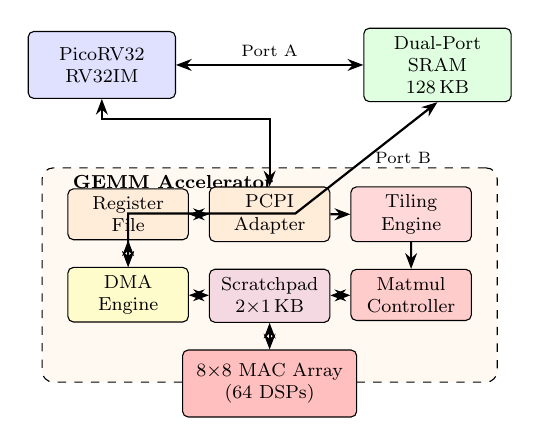
\begin{tikzpicture}[
    block/.style={draw, rounded corners=2pt, minimum height=0.7cm, minimum width=1.8cm, font=\footnotesize, align=center},
    bigblock/.style={draw, rounded corners=2pt, minimum height=1.0cm, minimum width=2.2cm, font=\footnotesize, align=center},
    arr/.style={-{Stealth[length=2mm]}, thick},
    darr/.style={{Stealth[length=2mm]}-{Stealth[length=2mm]}, thick},
    scale=0.85, transform shape
]
    % CPU
    \node[bigblock, fill=blue!12] (cpu) {PicoRV32\\RV32IM};

    % Memory
    \node[bigblock, fill=green!12, right=2.8cm of cpu] (mem) {Dual-Port\\SRAM\\128\,KB};

    % GEMM Accelerator box
    \node[draw, dashed, rounded corners=4pt, fill=orange!5,
          minimum width=6.8cm, minimum height=3.2cm,
          below=1.0cm of $(cpu.south)!0.5!(mem.south)$] (accelbox) {};
    \node[font=\footnotesize\bfseries, anchor=north west] at (accelbox.north west) {\quad GEMM Accelerator};

    % Internal blocks
    \node[block, fill=orange!15] at ($(accelbox.north)+(0,-0.7)$) (pcpi) {PCPI\\Adapter};
    \node[block, fill=orange!15, left=0.3cm of pcpi] (regfile) {Register\\File};
    \node[block, fill=red!15, right=0.3cm of pcpi] (tiling) {Tiling\\Engine};
    \node[block, fill=yellow!20, below=0.4cm of regfile] (dma) {DMA\\Engine};
    \node[block, fill=purple!15, below=0.4cm of pcpi] (spad) {Scratchpad\\2$\times$1\,KB};
    \node[block, fill=red!20, below=0.4cm of tiling] (ctrl) {Matmul\\Controller};
    \node[bigblock, fill=red!25, below=0.4cm of spad, minimum width=2.6cm] (mac) {8$\times$8 MAC Array\\(64 DSPs)};

    % Connections
    \draw[darr] (cpu.south) -- ++(0,-0.3) -| (pcpi.north);
    \draw[darr] (cpu.east) -- (mem.west) node[midway, above, font=\scriptsize] {Port A};
    \draw[darr] (dma.north) -- (regfile.south);
    \draw[arr] (tiling) -- (ctrl);
    \draw[darr] (spad) -- (ctrl);
    \draw[darr] (spad) -- (mac);
    \draw[darr] (dma) -- (spad);

    % DMA to memory
    \draw[darr] (dma.north) -- ++(0,0.8) -- ++(2.5,0) -- (mem.south) node[midway, right, font=\scriptsize] {Port B};

    % PCPI to regfile
    \draw[darr] (pcpi) -- (regfile);
    \draw[arr] (pcpi) -- (tiling);

\end{tikzpicture}
\caption{System-on-Chip architecture. The PicoRV32 CPU communicates with the GEMM accelerator via four custom PCPI instructions. The dual-port SRAM allows simultaneous CPU instruction fetch (Port~A) and DMA data transfer (Port~B) without arbitration.}
\label{fig:soc}
\end{figure}

\subsection{System Overview}

Fig.~\ref{fig:soc} shows the complete SoC. A PicoRV32 RISC-V core~\cite{picorv32} implementing the RV32IM instruction set is connected to a 128\,KB dual-port SRAM and the GEMM accelerator. The CPU accesses the accelerator through the Pico Co-Processor Interface (PCPI), which forwards unrecognized instructions to the accelerator's adapter module. The adapter decodes four custom R-type instructions encoded in the \texttt{custom-0} opcode space (Table~\ref{tab:instructions}).

The dual-port memory architecture eliminates bus arbitration: Port~A serves CPU instruction fetches and data accesses, while Port~B is dedicated to the DMA engine for matrix tile transfers. This ensures the CPU and accelerator never contend for memory bandwidth.

\subsection{MAC Unit and Systolic Array}

Each MAC unit is a two-stage pipelined multiply-accumulate datapath. Stage~1 performs the multiplication and registers the product; Stage~2 adds the product to a 48-bit accumulator. This allows one new input pair per clock cycle with a two-cycle latency.

The unit supports two precision modes controlled by a single \texttt{mode} signal:
\begin{itemize}
    \item \textbf{int8}: 8-bit $\times$ 8-bit $\rightarrow$ 16-bit product, accumulated in 48 bits.
    \item \textbf{int16}: 16-bit $\times$ 16-bit $\rightarrow$ 32-bit product, accumulated in 48 bits.
\end{itemize}
The 48-bit accumulator provides headroom for up to $2^{16}$ int8 accumulations without overflow. Saturation logic clamps the result if overflow occurs, preventing silent data corruption.

The 64 MAC units are arranged in an $8\times8$ grid using an \emph{output-stationary} dataflow. Each MAC ``owns'' one element of the output tile: MAC$(i,j)$ always computes $C[i][j]$. Input values are broadcast---row~$i$ of matrix~A feeds all columns, and column~$j$ of matrix~B feeds all rows---requiring only $8+8=16$ input values per cycle to keep all 64 units busy.

\subsection{Tiling Engine and Double-Buffered Scratchpad}

The tiling engine decomposes an arbitrary $M\times K \times N$ matrix multiplication into a grid of $8\times8$ tile operations, iterating in $K \rightarrow N \rightarrow M$ order. For non-aligned dimensions (e.g., $M=13$), it computes effective tile sizes (\texttt{eff\_m}, \texttt{eff\_k}, \texttt{eff\_n}) and passes them to the matmul controller, which adjusts its loop bounds accordingly.

The scratchpad consists of two 1\,KB SRAM banks operating in a ping-pong fashion. While the matmul controller reads from one bank to feed the MAC array, the DMA engine simultaneously writes the next tile into the other bank. A single-cycle \texttt{swap\_banks} pulse exchanges their roles. This overlapped load/compute strategy hides DMA latency and nearly doubles sustained throughput compared to a single-buffered design.

\subsection{DMA Engine}

The DMA engine transfers matrix tiles between the 128\,KB main memory and the scratchpad without CPU intervention. It supports configurable burst lengths (up to 16 words), reducing per-word overhead, and 2D strided access for extracting sub-blocks from row-major matrices. The 2D parameters---\texttt{x\_count} (words per row), \texttt{y\_count} (number of rows), \texttt{src\_stride}, \texttt{dst\_stride}---allow the engine to gather arbitrary rectangular regions in a single operation.

\subsection{32-Bit Accumulator Output Mode}

A key contribution is the \texttt{output\_acc32} control bit in the CTRL register. When set, the matmul controller writes the lower 32 bits of each 48-bit accumulator as a full 32-bit word to the scratchpad, rather than truncating to 8 or 16 bits.

This mode is critical for quantized neural network inference. In TFLite-style quantization, each layer's output must be \emph{requantized}:
\begin{equation}
    y_{\text{u8}} = \text{clamp}\!\left(\frac{\text{acc}_{32} \times M}{2^{S}},\ 0,\ 255\right)
    \label{eq:requant}
\end{equation}
where $M$ is a fixed-point multiplier and $S$ is a right-shift derived from the layer's quantization scales. Without access to the full accumulator, requantization must be precomputed offline. With \texttt{output\_acc32}, the CPU reads the raw 32-bit value and evaluates~(\ref{eq:requant}) using the RV32IM hardware \texttt{mul} instruction---entirely on-chip, with no offline tooling.

The acc32 mode incurs approximately $2\times$ DMA overhead (4 bytes per element vs.\ 1 byte in int8 mode) but delivers 23--100$\times$ speedup over software GEMM, making it practical for real-time inference.

% ============================================================
% IV. SOFTWARE STACK
% ============================================================
\section{Software Stack and Inference Pipeline}
\label{sec:software}

% --- Table I: Custom Instructions ---
\begin{table}[t]
\centering
\caption{Custom PCPI Instructions}
\label{tab:instructions}
\begin{tabular}{@{}llp{4.2cm}@{}}
\toprule
\textbf{Instruction} & \textbf{funct3} & \textbf{Description} \\
\midrule
\texttt{GEMM.CFG}    & 000 & Write \texttt{rs1} to accelerator register \texttt{rs2}; return old value in \texttt{rd}. \\
\texttt{GEMM.START}  & 001 & Assert start bit; return status. \\
\texttt{GEMM.WAIT}   & 010 & Stall CPU until accelerator completes; return cycle count. \\
\texttt{GEMM.STATUS} & 011 & Read status register (busy, done, error, overflow). \\
\bottomrule
\end{tabular}
\end{table}

\subsection{Driver API}

The bare-metal C driver exposes high-level functions that abstract the custom instructions. The primary entry points are:
\begin{itemize}
    \item \texttt{gemm\_run\_int8(M, K, N, ...)}: int8 GEMM with 8-bit output.
    \item \texttt{gemm\_run\_int8\_acc32(M, K, N, ...)}: int8 GEMM with 32-bit accumulator output.
\end{itemize}
Each function programs the 11 memory-mapped registers (dimensions, source/destination addresses, row strides), atomically sets the mode bits and start bit via a single \texttt{GEMM.CFG} write, and blocks until completion via \texttt{GEMM.WAIT}.

All row strides must be aligned to 4-byte boundaries for the DMA engine. The driver provides a \texttt{PAD4(x)} macro that rounds up to the nearest multiple of~4.

\subsection{Neural Network Inference Pipeline}

% --- Fig 2: Inference Pipeline ---
\begin{figure}[t]
\centering
\begin{tikzpicture}[
    step/.style={draw, rounded corners=2pt, minimum height=0.6cm, minimum width=2.0cm, font=\footnotesize, align=center},
    arr/.style={-{Stealth[length=2mm]}, thick},
    cpucolor/.style={fill=blue!12},
    hwcolor/.style={fill=red!15},
    scale=0.85, transform shape
]
    \node[step, cpucolor] (im2col) {im2col\\(CPU)};
    \node[step, hwcolor, right=0.6cm of im2col] (gemm) {GEMM acc32\\(Accelerator)};
    \node[step, cpucolor, right=0.6cm of gemm] (requant) {Requantize\\(CPU: mul+shift)};
    \node[step, cpucolor, right=0.6cm of requant] (relu) {ReLU\\(CPU)};

    \draw[arr] (im2col) -- (gemm);
    \draw[arr] (gemm) -- (requant) node[midway, above, font=\scriptsize] {32-bit};
    \draw[arr] (requant) -- (relu) node[midway, above, font=\scriptsize] {uint8};

    \node[font=\scriptsize, below=0.15cm of im2col] {Rearrange};
    \node[font=\scriptsize, below=0.15cm of gemm] {64 MACs/cyc};
    \node[font=\scriptsize, below=0.15cm of requant] {$\frac{a \times M}{2^S}$};
    \node[font=\scriptsize, below=0.15cm of relu] {clamp $\geq 0$};
\end{tikzpicture}
\caption{Per-layer inference pipeline. Blue blocks execute on the RV32IM CPU; red on the accelerator. The 32-bit accumulator flows to the CPU for fixed-point requantization.}
\label{fig:pipeline}
\end{figure}

Fig.~\ref{fig:pipeline} illustrates the per-layer inference flow for a quantized convolutional neural network. For each layer:

\begin{enumerate}
    \item \textbf{im2col} (CPU): The input feature map is rearranged into a column matrix so that convolution reduces to GEMM.
    \item \textbf{GEMM} (Accelerator): The hardware computes $C = A \times B$ in \texttt{acc32} mode, writing full 32-bit accumulators to memory.
    \item \textbf{Requantize} (CPU): The CPU reads each 32-bit value and applies fixed-point scaling: $y = \text{clamp}((a \times M) \gg S,\, 0,\, 255)$ using the RV32IM hardware multiplier.
    \item \textbf{ReLU} (CPU): Activation function (a no-op for unsigned uint8 in the common case).
\end{enumerate}

This pipeline requires \emph{no offline precomputation}. The requantization parameters ($M$, $S$) are embedded in the firmware as compile-time constants derived from the model's quantization scales.

\subsection{MNIST Case Study}

We demonstrate the full pipeline on a TFLite-quantized MNIST classifier:
\begin{itemize}
    \item Conv2D($1 {\rightarrow} 8$, $3{\times}3$, stride~2) $\rightarrow$ 13$\times$13$\times$8
    \item Conv2D($8 {\rightarrow} 16$, $3{\times}3$, stride~2) $\rightarrow$ 6$\times$6$\times$16
    \item FC($576 {\rightarrow} 10$) $\rightarrow$ 10 logits $\rightarrow$ argmax
\end{itemize}
All GEMM operations use \texttt{acc32} mode with CPU-side requantization. Three test images (digits 7, 2, 1) are classified correctly, with all 9 GEMM layer outputs matching the Python golden model bit-exactly.

% ============================================================
% V. EXPERIMENTAL RESULTS
% ============================================================
\section{Experimental Results}
\label{sec:results}

All results are obtained using Xilinx Vivado~2024.2 targeting the Artix-7 \texttt{xc7a100tcsg324-1} FPGA. Functional verification uses Icarus Verilog with bit-exact comparison against NumPy golden models.

\subsection{FPGA Resource Utilization}

% --- Table II: Utilization ---
\begin{table}[t]
\centering
\caption{FPGA Resource Utilization (Post-Route)}
\label{tab:utilization}
\begin{tabular}{@{}lrrr@{}}
\toprule
\textbf{Resource} & \textbf{Accel.} & \textbf{Full SoC} & \textbf{\% of xc7a100t} \\
\midrule
Slice LUTs         & 5{,}226 & 6{,}287 &  9.92\% \\
Flip-Flops         & 6{,}362 & 7{,}094 &  5.59\% \\
Block RAM (36Kb)   &       2 &      34 & 25.19\% \\
DSP48E1            &      70 &      70 & 29.17\% \\
\midrule
\multicolumn{2}{@{}l}{Clock frequency (Fmax)} & \multicolumn{2}{r}{91.7\,MHz} \\
\multicolumn{2}{@{}l}{WNS at 100\,MHz target} & \multicolumn{2}{r}{$-$0.906\,ns} \\
\bottomrule
\end{tabular}
\end{table}

% --- Table III: Hierarchical Breakdown ---
\begin{table}[t]
\centering
\caption{Hierarchical Resource Breakdown}
\label{tab:hier}
\begin{tabular}{@{}lrrr@{}}
\toprule
\textbf{Module} & \textbf{LUTs} & \textbf{FFs} & \textbf{DSPs} \\
\midrule
MAC Array ($8\times8$) & 2{,}793 & 4{,}184 & 64 \\
Matmul Controller      & 1{,}352 & 1{,}248 &  0 \\
Tiling Engine          &     423 &     272 &  6 \\
DMA Engine             &     302 &     243 &  0 \\
Register File          &     243 &     322 &  0 \\
PCPI Adapter           &     158 &      92 &  0 \\
Scratchpad (2$\times$1\,KB) &  64 &       1 &  0 \\
\midrule
\textbf{Accelerator total} & \textbf{5{,}226} & \textbf{6{,}362} & \textbf{70} \\
PicoRV32 CPU           & 1{,}060 &     609 &  0 \\
Main Memory (128\,KB)  &       0 &       0 & 32\,BRAM \\
\bottomrule
\end{tabular}
\end{table}

Table~\ref{tab:utilization} reports post-route utilization for the complete SoC. The entire design fits in under 10\% of the Artix-7 LUTs, leaving ample room for additional peripherals. The 34 Block RAMs are dominated by the 128\,KB main memory (32 RAMB36E1); the accelerator itself uses only 2 BRAMs for the scratchpad.

Table~\ref{tab:hier} provides a per-module breakdown. The $8\times8$ MAC array consumes the most logic (2{,}793 LUTs, 64 DSPs), followed by the matmul controller (1{,}352 LUTs) which handles data unpacking and write-back. The tiling engine, despite its complexity, requires only 423 LUTs.

The design achieves an estimated Fmax of 91.7\,MHz with a worst negative slack of $-$0.906\,ns at the 100\,MHz target. Timing closure at 100\,MHz is achievable with additional pipelining in the critical path.

\subsection{Performance}

% --- Table IV: Benchmark Results ---
\begin{table}[t]
\centering
\caption{GEMM Benchmark: Software vs.\ Hardware}
\label{tab:benchmark}
\begin{tabular}{@{}rrrrrr@{}}
\toprule
\textbf{Size} & \textbf{SW} & \multicolumn{2}{c}{\textbf{int8 mode}} & \multicolumn{2}{c}{\textbf{acc32 mode}} \\
\cmidrule(lr){3-4} \cmidrule(lr){5-6}
 & \textbf{Cycles} & \textbf{Cycles} & \textbf{Speedup} & \textbf{Cycles} & \textbf{Speedup} \\
\midrule
$4{\times}4$   &   4{,}775 &    127 &  37.6$\times$ &    211 & 22.9$\times$ \\
$5{\times}5$   &   8{,}859 &    178 &  49.8$\times$ &    283 & 31.5$\times$ \\
$7{\times}7$   &  22{,}979 &    240 &  95.7$\times$ &    457 & 50.5$\times$ \\
$8{\times}8$   &  33{,}723 &    271 & 124.4$\times$ &    559 & 60.5$\times$ \\
$10{\times}10$ &  64{,}349 &    820 &  78.5$\times$ & 1{,}375 & 46.9$\times$ \\
$13{\times}13$ & 138{,}443 & 1{,}029 & 134.5$\times$ & 1{,}907 & 72.7$\times$ \\
$16{\times}16$ & 254{,}819 & 1{,}202 & 212.0$\times$ & 2{,}546 & 100.2$\times$ \\
\bottomrule
\end{tabular}
\end{table}

% --- Fig 3: Speedup Bar Chart ---
\begin{figure}[t]
\centering
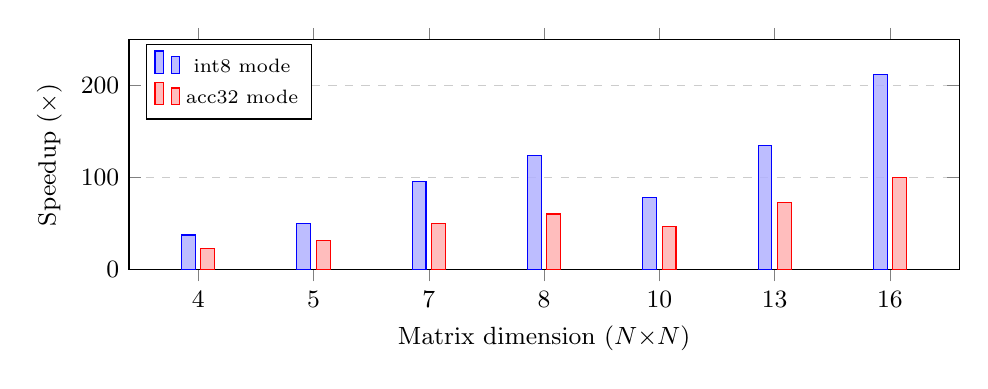
\begin{tikzpicture}
\begin{axis}[
    ybar,
    bar width=5pt,
    width=\columnwidth,
    height=4.5cm,
    ylabel={Speedup ($\times$)},
    xlabel={Matrix dimension ($N{\times}N$)},
    symbolic x coords={4,5,7,8,10,13,16},
    xtick=data,
    ymin=0, ymax=250,
    legend style={at={(0.02,0.98)}, anchor=north west, font=\scriptsize},
    ymajorgrids=true,
    grid style={dashed, gray!40},
    tick label style={font=\small},
    label style={font=\small},
    every axis plot/.append style={fill opacity=0.85},
]
\addplot coordinates {(4,37.6) (5,49.8) (7,95.7) (8,124.4) (10,78.5) (13,134.5) (16,212.0)};
\addplot coordinates {(4,22.9) (5,31.5) (7,50.5) (8,60.5) (10,46.9) (13,72.7) (16,100.2)};
\legend{int8 mode, acc32 mode}
\end{axis}
\end{tikzpicture}
\caption{Speedup over software GEMM on PicoRV32 RV32IM. The dip at $10{\times}10$ is caused by non-aligned tiling (10 is not a multiple of~8), which introduces partial tiles and extra DMA passes.}
\label{fig:speedup}
\end{figure}

Table~\ref{tab:benchmark} and Fig.~\ref{fig:speedup} compare software and hardware GEMM performance. The software baseline is a triple-nested loop compiled with \texttt{-Os} on RV32IM (with hardware multiply). Key observations:

\begin{itemize}
    \item Speedup increases with matrix size as DMA and control overhead is amortized over more computation. At $16{\times}16$, the accelerator is 212$\times$ faster in int8 mode.
    \item The \texttt{acc32} mode is approximately $2\times$ slower than int8 due to $4\times$ more DMA store traffic, but still delivers 23--100$\times$ speedup---more than sufficient for real-time inference.
    \item The dip at $10{\times}10$ results from non-aligned tiling: dimension~10 requires two tile passes along each axis (one full $8{\times}8$ tile plus one $2$-wide partial tile), reducing MAC utilization.
\end{itemize}

For neural network layers, the Conv2D benchmark achieves 35.1$\times$ speedup (including im2col overhead on the CPU), and the FC layer achieves 7.3$\times$ (dominated by small matrix size).

\subsection{Power Analysis}

% --- Fig 4: Power Breakdown ---
\begin{figure}[t]
\centering
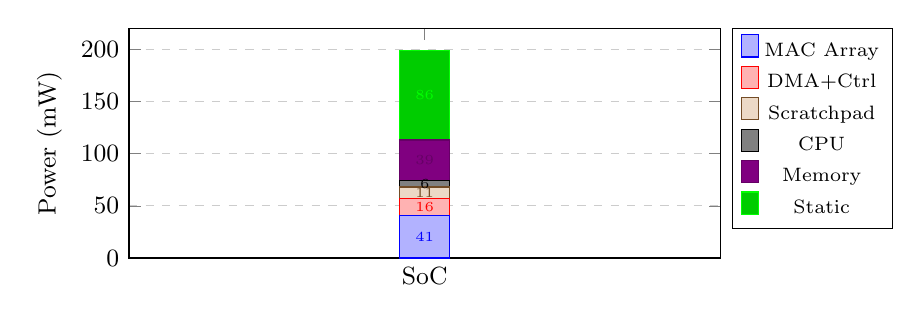
\begin{tikzpicture}
\begin{axis}[
    ybar stacked,
    bar width=18pt,
    width=0.75\columnwidth,
    height=4.5cm,
    ylabel={Power (mW)},
    symbolic x coords={SoC},
    xtick=data,
    ymin=0, ymax=220,
    legend style={at={(1.02,1.0)}, anchor=north west, font=\scriptsize},
    ymajorgrids=true,
    grid style={dashed, gray!40},
    tick label style={font=\small},
    label style={font=\small},
    nodes near coords,
    every node near coord/.append style={font=\tiny},
]
\addplot coordinates {(SoC,41)};
\addplot coordinates {(SoC,16)};
\addplot coordinates {(SoC,11)};
\addplot coordinates {(SoC,6)};
\addplot coordinates {(SoC,39)};
\addplot coordinates {(SoC,86)};
\legend{MAC Array, DMA+Ctrl, Scratchpad, CPU, Memory, Static}
\end{axis}
\end{tikzpicture}
\caption{Power breakdown of the full SoC (199\,mW total). Static FPGA leakage accounts for 86\,mW; the accelerator's dynamic power is 68\,mW.}
\label{fig:power}
\end{figure}

Fig.~\ref{fig:power} shows the power breakdown from Vivado's post-route power analysis. The total on-chip power is 199\,mW, of which 86\,mW is static FPGA leakage (inherent to the device). The accelerator's dynamic power is 68\,mW, dominated by the MAC array (41\,mW) and scratchpad+DMA (27\,mW combined). The PicoRV32 CPU adds only 6\,mW.

\subsection{Energy Efficiency}

The peak compute throughput is:
\begin{equation}
    64 \text{ MACs/cycle} \times 91.7\text{\,MHz} = 5.87\text{\,GOPS}
\end{equation}
The energy efficiency is:
\begin{equation}
    \frac{5.87\text{\,GOPS}}{0.113\text{\,W (dynamic)}} \approx 52\text{\,GOPS/W}
\end{equation}
This is competitive with ASIC designs such as Eyeriss ($\sim$10\,GOPS/W in 65\,nm), noting that FPGA implementations incur substantial overhead from programmable routing and configurable logic.

\subsection{Comparison with Prior Work}

% --- Table V: Comparison ---
\begin{table}[t]
\centering
\caption{Comparison with Related Accelerators}
\label{tab:comparison}
\begin{tabular}{@{}lcccc@{}}
\toprule
& \textbf{This} & \textbf{Eyeriss} & \textbf{Edge} & \textbf{Gemmini} \\
& \textbf{work} & \textbf{v1}~\cite{chen2017eyeriss} & \textbf{TPU}~\cite{edgetpu} & \cite{genc2021gemmini} \\
\midrule
Technology & Artix-7 & 65\,nm & 40\,nm & FPGA \\
& FPGA & ASIC & ASIC & (various) \\
Array size & $8{\times}8$ & $14{\times}12$ & $256{\times}256$ & Config. \\
Precision & int8/16 & int16 & int8 & int8 \\
Frequency & 92\,MHz & 200\,MHz & --- & $\sim$50\,MHz \\
Power & 199\,mW & 278\,mW & 2\,W & --- \\
Eff. (GOPS/W) & 52 & $\sim$10 & $\sim$2{,}000 & --- \\
On-chip & \checkmark & --- & --- & \checkmark \\
\quad requant. & & & & \\
Open source & \checkmark & --- & --- & \checkmark \\
RISC-V & \checkmark & --- & --- & \checkmark \\
\quad integrated & & & & \\
\bottomrule
\end{tabular}
\end{table}

Table~\ref{tab:comparison} positions our design among related accelerators. Our work occupies a distinct niche: the smallest viable GEMM co-processor with RISC-V integration, on-chip requantization, and complete open-source RTL. The FPGA-based energy efficiency (52\,GOPS/W) would improve substantially in an ASIC implementation, where static power and routing overhead are eliminated.

\subsection{Verification}

The design is verified at four levels:
\begin{enumerate}
    \item \textbf{Unit}: Individual MAC unit, array, DMA, scratchpad, and controller testbenches.
    \item \textbf{Integration}: Full accelerator pipeline with multi-tile and non-aligned matrices.
    \item \textbf{System}: PicoRV32 boots C firmware, executes GEMM via custom instructions, and verifies results against embedded golden checksums.
    \item \textbf{Application}: Complete MNIST CNN inference with three test images.
\end{enumerate}

In total, 60 test patterns (31 stress tests, 14 benchmarks, 6 NN layer tests, 9 MNIST GEMM layers) pass with zero mismatches against Python golden models.

% ============================================================
% VI. CONCLUSION
% ============================================================
\section{Conclusion and Future Work}
\label{sec:conclusion}

We presented an energy-efficient RISC-V GEMM co-processor for edge AI inference, featuring an $8\times8$ output-stationary MAC array, autonomous hardware tiling with overlapped DMA, and a 32-bit accumulator output mode that enables on-chip requantization without offline precomputation. The complete SoC, implemented on an Artix-7 FPGA, achieves up to 212$\times$ speedup over software at 199\,mW total power, using under 10\% of the FPGA's logic resources. End-to-end MNIST digit recognition with a TFLite-quantized CNN demonstrates practical applicability.

Future directions include: (i)~ASIC tape-out for accurate power characterization without FPGA overhead; (ii)~scaling to $16{\times}16$ arrays for higher throughput; (iii)~a dedicated hardware requantization unit to offload the shift-scale operation from the CPU; (iv)~sparsity-aware computation to skip zero-valued multiplications; and (v)~integration with the TFLite Micro runtime as a transparent GEMM backend.

% ============================================================
% REFERENCES
% ============================================================
\balance
\begin{thebibliography}{00}

\bibitem{banbury2021mlperf}
C.~Banbury \emph{et~al.}, ``MLPerf Tiny Benchmark,'' in \emph{Proc.\ NeurIPS Datasets and Benchmarks Track}, 2021.

\bibitem{jouppi2017datacenter}
N.~P.~Jouppi \emph{et~al.}, ``In-datacenter performance analysis of a tensor processing unit,'' in \emph{Proc.\ ACM/IEEE ISCA}, 2017, pp.~1--12.

\bibitem{tflite}
R.~David \emph{et~al.}, ``TensorFlow Lite Micro: Embedded machine learning for TinyML systems,'' in \emph{Proc.\ MLSys}, 2021.

\bibitem{edgetpu}
Google, ``Edge TPU: Google's purpose-built ASIC for ML inference at the edge,'' \url{https://cloud.google.com/edge-tpu}, 2019.

\bibitem{chen2017eyeriss}
Y.-H.~Chen, J.~Emer, and V.~Sze, ``Eyeriss: An energy-efficient reconfigurable accelerator for deep convolutional neural networks,'' \emph{IEEE J.\ Solid-State Circuits}, vol.~52, no.~1, pp.~127--138, Jan.\ 2017.

\bibitem{chen2019eyeriss}
Y.-H.~Chen \emph{et~al.}, ``Eyeriss v2: A flexible accelerator for emerging deep neural networks on mobile devices,'' \emph{IEEE J.\ Emerging and Selected Topics in Circuits and Systems}, vol.~9, no.~2, pp.~292--308, Jun.\ 2019.

\bibitem{genc2021gemmini}
H.~Genc \emph{et~al.}, ``Gemmini: Enabling systematic deep-learning architecture evaluation via full-stack integration,'' in \emph{Proc.\ ACM/IEEE DAC}, 2021, pp.~769--774.

\bibitem{cfu}
Google, ``CFU Playground: Full-stack open-source framework for tiny machine learning,'' \url{https://cfu-playground.readthedocs.io}, 2022.

\bibitem{nvdla}
NVIDIA, ``NVDLA: Open-source deep learning accelerator,'' \url{http://nvdla.org}, 2018.

\bibitem{picorv32}
C.~Wolf, ``PicoRV32 -- A size-optimized RISC-V CPU,'' \url{https://github.com/YosysHQ/picorv32}, 2023.

\end{thebibliography}

\end{document}
